\documentclass[conference]{IEEEtran}
\IEEEoverridecommandlockouts

\usepackage{cite}
\usepackage{amsmath,amssymb,amsfonts}
\usepackage{algorithmic}
\usepackage{algorithm}
\usepackage{graphicx}
\usepackage{textcomp}
\usepackage{xcolor}
\usepackage{booktabs}
\usepackage{multirow}
\usepackage{hyperref}

\graphicspath{{../../plots/}}

\begin{document}

\title{LOS/NLOS Classification and Distance Estimation for UWB Indoor Positioning Using Feature-Engineered ML and Hybrid CNN-Transformer}

\author{
\IEEEauthorblockN{Po Haoting, Travis Neo Kuang Yi, Chiang Porntep, Nico Caleb Lim, and Dui Ru En Joshua}
\IEEEauthorblockA{\textit{Lab P1, Group 4, School of Computing} \\
\textit{Singapore Institute of Technology and University of Glasgow}\\
Singapore}
}

\maketitle

\begin{abstract}
Accurate line-of-sight (LOS) and non-line-of-sight (NLOS) identification is essential for precise ultra-wideband (UWB) indoor positioning. We study a concise dual-pipeline framework for two-path LOS/NLOS classification and distance estimation using the Decawave DWM1000 dataset. After preprocessing, 40,864 second paths are recovered from 41,996 valid CIR measurements, yielding an expanded two-path dataset of 83,992 rows for the feature-engineered pipeline. Among classical models, XGBoost achieves the best classification performance (accuracy 0.9404, AUC 0.9834), while simple and stacked ensembles provide only marginal gains. A separate raw-CIR CNN+Transformer pipeline reaches AUC 0.9821 on the original split, and 0.9845 with CIR augmentation in that separate pipeline. For distance estimation, path~1 regression remains moderate (best RMSE 1.3706\,m, $R^2=0.6698$), whereas path~2 regression appears nearly perfect because the target is analytically derived from features that include RANGE and path timing. Unsupervised clustering is weak (K-Means accuracy 0.5906, ARI 0.0269; DBSCAN labels all test points as noise), so it should not be overstated.
\end{abstract}

\begin{IEEEkeywords}
UWB, LOS/NLOS classification, channel impulse response, CNN, Transformer, indoor positioning, distance estimation
\end{IEEEkeywords}

%======================================================================
\section{Introduction}

Ultra-wideband (UWB) technology has emerged as a leading solution for centimeter-level indoor positioning due to its high time resolution and resistance to multipath fading~\cite{b1}. However, NLOS propagation conditions cause systematic ranging errors that severely degrade positioning accuracy. Identifying whether a signal travels via LOS or NLOS is therefore critical for mitigating these errors~\cite{b2}.

The channel impulse response (CIR) recorded by UWB receivers encodes rich information about the propagation environment. Traditional approaches extract hand-crafted features such as rise time, kurtosis, and energy ratios from the CIR, then apply classifiers like support vector machines (SVM), k-nearest neighbors, or random forests~\cite{b3,b4}. While effective, these methods rely on domain expertise for feature selection and may miss subtle signal patterns.

Recent advances in deep learning offer an alternative: learning discriminative features directly from raw waveforms. Convolutional neural networks (CNNs) have been applied to UWB CIR classification~\cite{b5}, but they capture only local patterns. Transformer architectures~\cite{b6} excel at modeling long-range dependencies through self-attention, making them well-suited for analyzing the full CIR waveform where multipath components may be widely separated. Prior work has already applied transformers to UWB NLOS detection, including a Transformer-based model on the same Bregar dataset~\cite{b11} and a transformer-convolutional architecture for UWB NLOS classification~\cite{b12}.

However, most existing studies focus on binary LOS/NLOS classification of a single propagation path. In realistic indoor environments, UWB signals arrive via multiple paths, and identifying the propagation condition of secondary reflections is equally important for multipath-aided positioning~\cite{b3}. Furthermore, fewer studies compare a two-path feature-engineered pipeline directly against an end-to-end raw-CIR deep model within one evaluation framework. XGBoost~\cite{b8}, a state-of-the-art gradient boosting framework, has shown strong performance in similar classification tasks but has not been extensively applied to UWB CIR analysis.

In this paper, we make the following contributions:
\begin{itemize}
    \item A two-path extraction and labeling framework that extends binary LOS/NLOS classification to the two dominant signal paths in each CIR measurement.
    \item A feature engineering pipeline producing 25 per-path features for classical ML models.
    \item A hybrid 1D-CNN + Transformer architecture that operates directly on the raw 1016-sample CIR waveform, achieving classification performance matching hand-crafted features.
    \item Distance estimation models for both dominant paths, with a clearer assessment of the differing difficulty of path~1 and path~2 targets.
\end{itemize}

%======================================================================
\section{Dataset and Data Preparation}

\subsection{Dataset Description}

We use the publicly available UWB LOS/NLOS dataset~\cite{b7} collected using Decawave DWM1000 modules across seven distinct indoor environments. The dataset contains 42,000 samples (21,000 LOS and 21,000 NLOS), each comprising 14 scalar features and a 1016-sample CIR recorded at 1\,ns resolution. Table~\ref{tab:features} summarizes the key features.

\begin{table}[t]
\caption{Dataset Features}
\label{tab:features}
\centering
\begin{tabular}{@{}ll@{}}
\toprule
\textbf{Feature} & \textbf{Description} \\
\midrule
RANGE & Measured distance (m) \\
FP\_IDX & First path index in CIR \\
FP\_AMP1--3 & First path amplitude estimators \\
STDEV\_NOISE & Standard deviation of noise \\
CIR\_PWR & Total CIR power \\
MAX\_NOISE & Maximum noise level \\
RXPACC & Preamble accumulation count \\
FRAME\_LEN & Frame length \\
PREAM\_LEN & Preamble length \\
CIR0--CIR1015 & 1016-sample channel impulse response \\
\bottomrule
\end{tabular}
\end{table}

\subsection{Data Preparation}

Our preprocessing pipeline performs the following steps:

\textbf{CIR normalization.} Each CIR sample is divided by its corresponding RXPACC value to normalize the preamble accumulation effect, as specified in the DWM1000 documentation.

\textbf{Constant column removal.} Three features (CH, BITRATE, PRFR) have identical values across all 42,000 samples and are removed, reducing the scalar feature set from 14 to 11.

\textbf{Feature scaling.} The 11 remaining scalar features are standardized using zero-mean unit-variance scaling (StandardScaler).

\textbf{NaN/Inf handling.} Any NaN or Inf values introduced during CIR normalization are replaced with zero.

\textbf{Outlier analysis and retention.} Tukey IQR analysis was performed on all 11 retained scalar features. Overall, 16.9\% of samples are outliers in at least one scalar feature, but most were retained because many correspond to genuine NLOS behavior rather than sensor faults. For example, FP\_IDX outliers are 98.7\% NLOS and RANGE outliers are 100\% NLOS, indicating physically meaningful delayed arrivals and large ranging bias. Only 4 degenerate samples with RANGE$=0$ or CIR\_PWR$=0$ were removed as likely hardware errors, leaving 41,996 valid samples. This retention strategy is appropriate because the main supervised models are tree-based and robust to outliers, while StandardScaler mitigates scale effects for the deep model and for distance-based clustering.

\textbf{Train/test split.} The dataset is divided using stratified 80/20 splitting to preserve class balance.

Fig.~\ref{fig:class_dist} confirms the balanced class distribution (50/50 LOS/NLOS). Fig.~\ref{fig:distributions} shows the distribution of key features by LOS/NLOS class, revealing clear separability for several features. Fig.~\ref{fig:correlation} shows inter-feature correlations.

\begin{figure}[t]
\centering
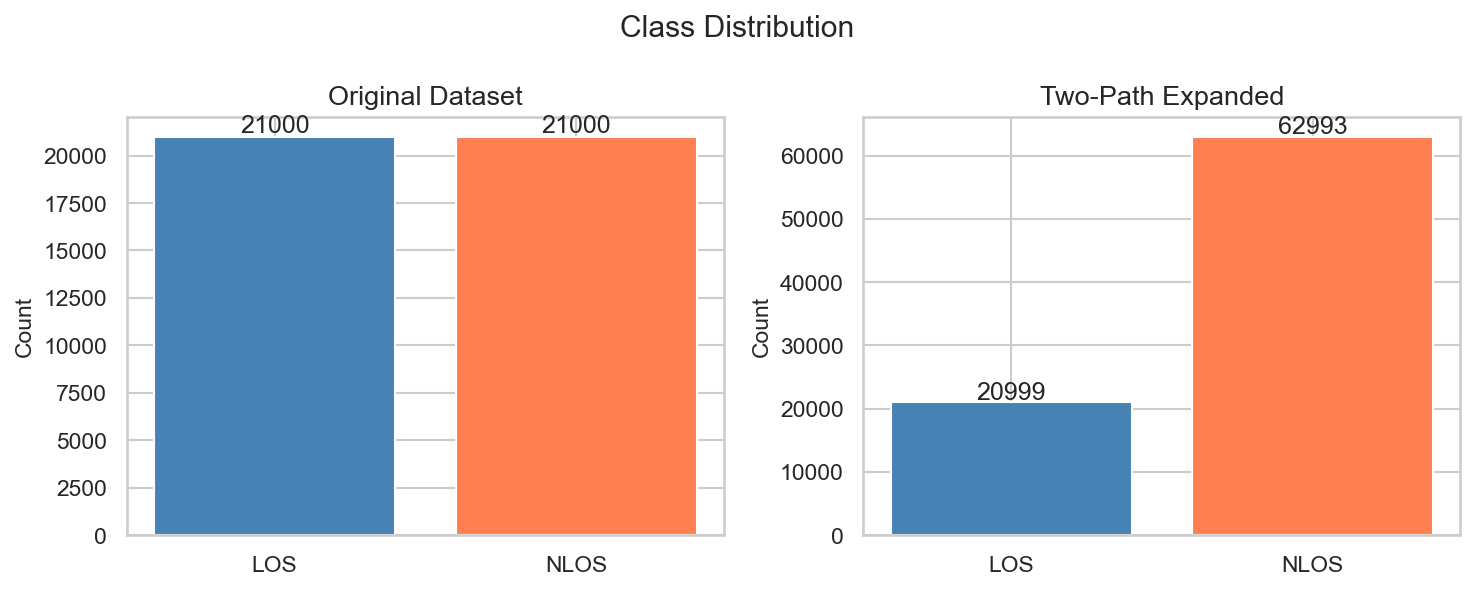
\includegraphics[width=\columnwidth]{01_class_distribution.png}
\caption{Class distribution of the original dataset showing balanced LOS and NLOS samples (21,000 each).}
\label{fig:class_dist}
\end{figure}

\begin{figure}[t]
\centering
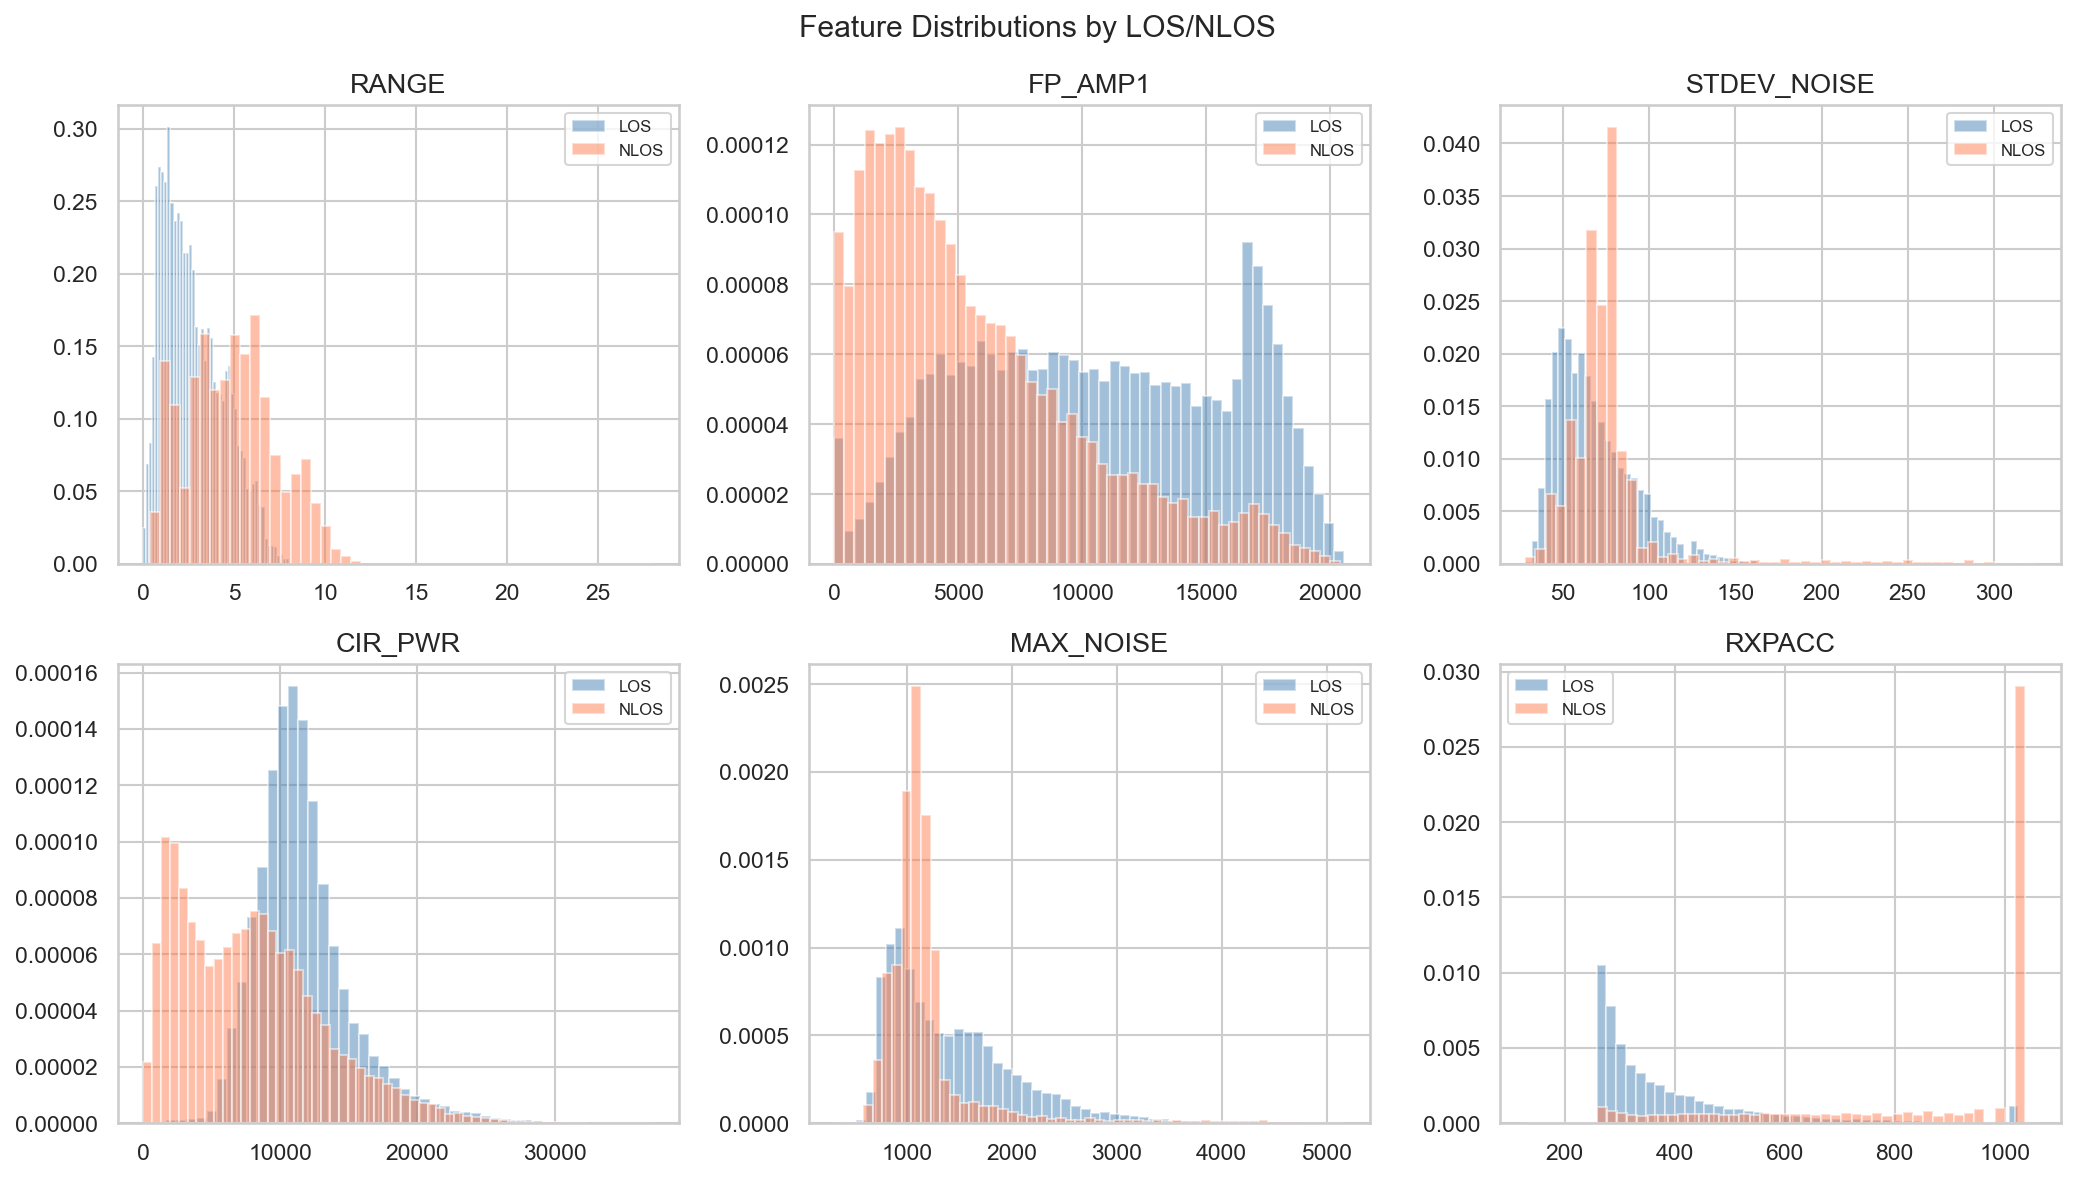
\includegraphics[width=\columnwidth]{02_feature_distributions.png}
\caption{Distribution of scalar features by LOS (blue) and NLOS (orange) class. Features such as CIR\_PWR and FP\_AMP1 show strong class separability.}
\label{fig:distributions}
\end{figure}

\begin{figure}[t]
\centering
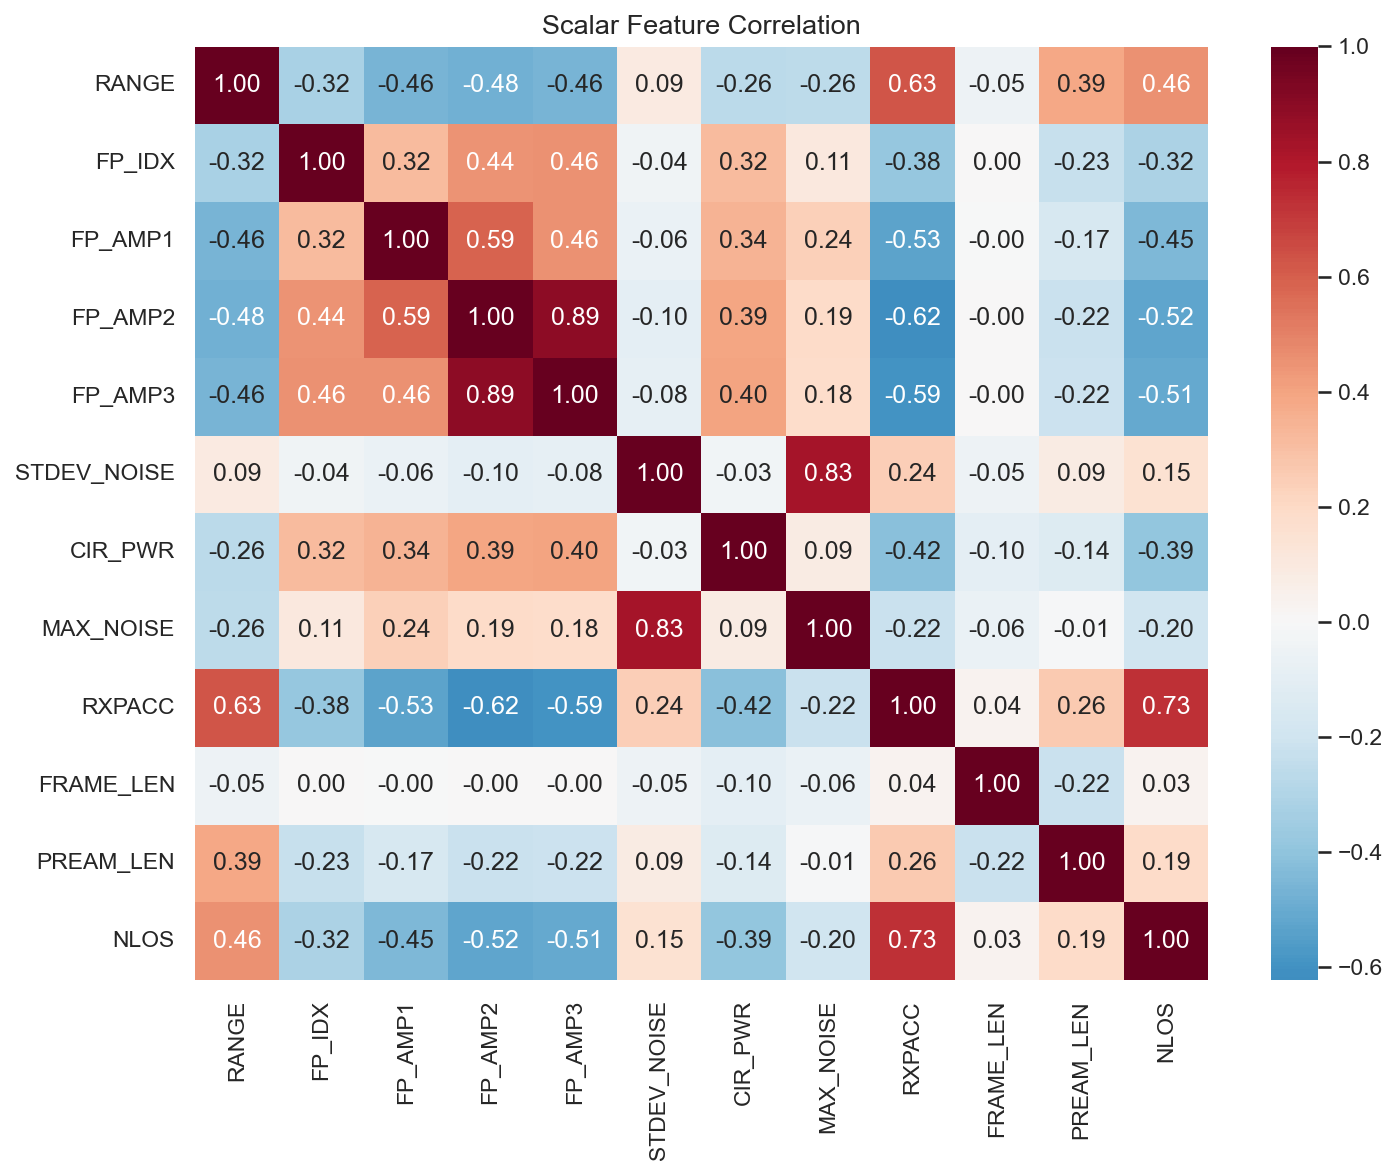
\includegraphics[width=\columnwidth]{03_correlation_heatmap.png}
\caption{Pearson correlation matrix of 11 scalar features. High correlation among FP\_AMP1--3 suggests potential for dimensionality reduction.}
\label{fig:correlation}
\end{figure}

%======================================================================
\section{Proposed Methodology}

\subsection{Two-Path Extraction}

UWB CIR measurements often contain multiple propagation paths. The two shortest (dominant) paths carry the most information for positioning: if the first path is LOS, the second is necessarily NLOS (reflected); if the first path is NLOS, both paths are NLOS. Algorithm~\ref{alg:peak} describes our peak detection procedure.

\begin{algorithm}[t]
\caption{Two-Path Peak Detection}
\label{alg:peak}
\begin{algorithmic}[1]
\REQUIRE CIR waveform $c[0..1015]$, first path index $\mathrm{FP\_IDX}$
\ENSURE Path indices $p_1, p_2$ and amplitudes $a_1, a_2$
\STATE $p_1 \leftarrow \arg\max_{j \in [\mathrm{FP\_IDX}-10, \mathrm{FP\_IDX}+10]} c[j]$
\STATE $a_1 \leftarrow c[p_1]$
\STATE Find all peaks in $c$ with height $> 0.1 \cdot a_1$, distance $> 15$, prominence $> 0.05 \cdot a_1$
\STATE Remove peaks within $\pm 20$ samples of $p_1$
\STATE $p_2 \leftarrow$ index of strongest remaining peak
\STATE $a_2 \leftarrow c[p_2]$
\RETURN $p_1, a_1, p_2, a_2$
\end{algorithmic}
\end{algorithm}

Applying this algorithm after preprocessing, a second path is detected in 40,864 of 41,996 samples (97.3\%). Fig.~\ref{fig:fp_idx} shows the FP\_IDX distribution by class, and Fig.~\ref{fig:cir} shows example CIR waveforms with detected peaks.

\begin{figure}[t]
\centering
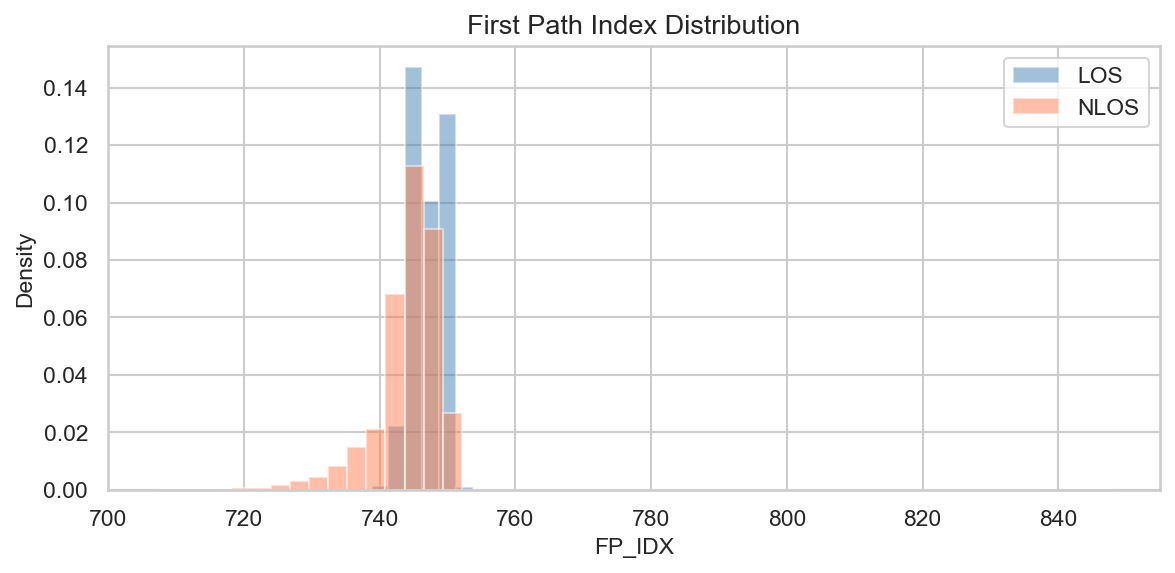
\includegraphics[width=\columnwidth]{05_fp_idx_distribution.png}
\caption{Distribution of first path index (FP\_IDX) by LOS and NLOS class. NLOS signals exhibit later and more variable first path arrival.}
\label{fig:fp_idx}
\end{figure}

\textbf{Two-path labeling.} For each valid original sample, we generate two rows: path~1 retains the original LOS/NLOS label; path~2 is always labeled NLOS (since any secondary reflection is, by definition, not the direct path). This yields an expanded dataset of 83,992 rows.

\begin{figure}[t]
\centering
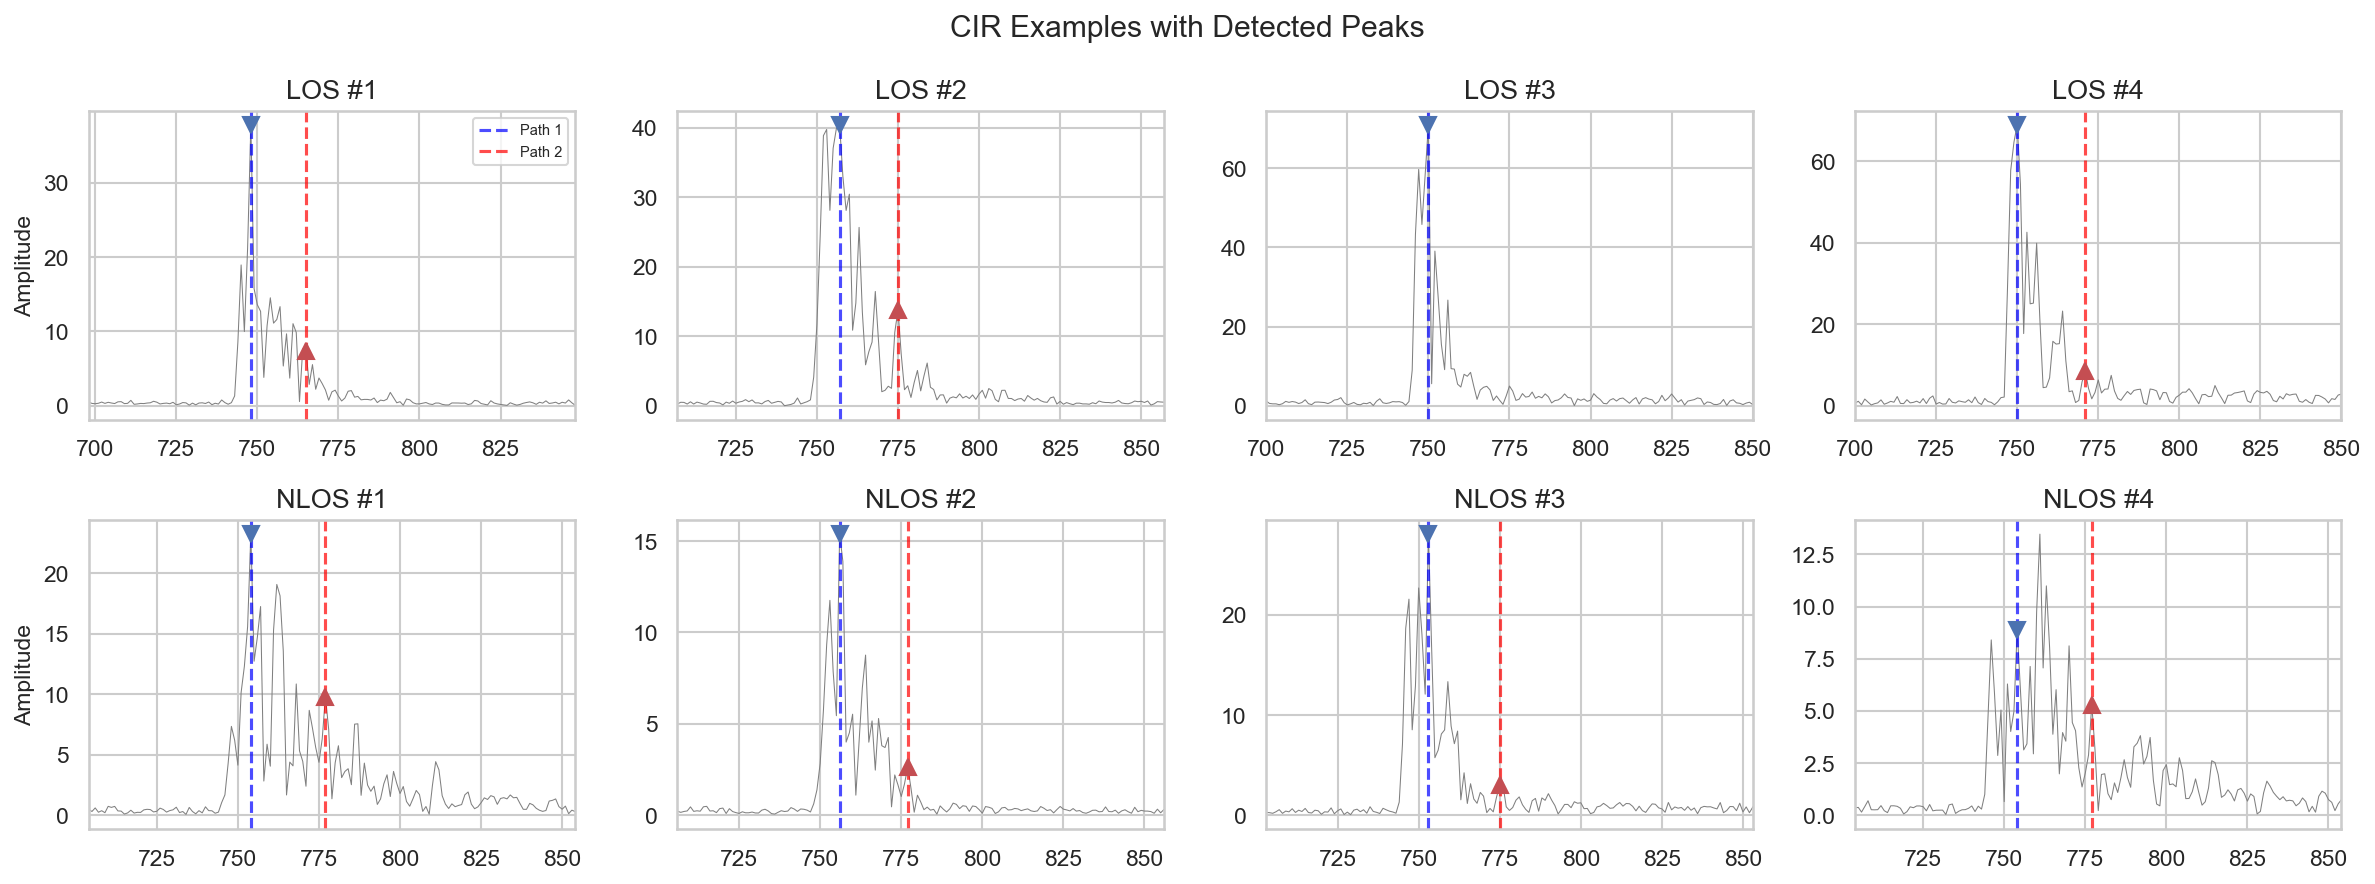
\includegraphics[width=\columnwidth]{04_cir_examples.png}
\caption{Example CIR waveforms showing detected first path (triangle) and second path (circle) for LOS and NLOS conditions.}
\label{fig:cir}
\end{figure}

\subsection{Feature Engineering Pipeline}

For each detected path, we compute 8 local waveform features (Table~\ref{tab:path_features}) together with 5 full-CIR statistical descriptors, 9 shared scalar features, and 3 derived shared features, yielding a 25-dimensional feature vector per path.

\begin{table}[t]
\caption{Key local per-path engineered features (8 of the 13 per-path descriptors)}
\label{tab:path_features}
\centering
\begin{tabular}{@{}ll@{}}
\toprule
\textbf{Feature} & \textbf{Description} \\
\midrule
path\_idx & Peak sample index in CIR \\
path\_amp & Peak amplitude \\
rise\_time & Samples from 10\% threshold to peak \\
decay\_time & Samples from peak to 10\% threshold \\
kurtosis\_local & Kurtosis of $\pm$15-sample window \\
energy\_ratio & Local energy / total CIR energy \\
peak\_to\_noise & Peak amplitude / STDEV\_NOISE \\
amplitude\_ratio & This path amp / other path amp \\
\bottomrule
\end{tabular}
\end{table}

Feature importance ranking and RFECV both indicate that the strongest signal is concentrated in a very small subset of path descriptors. In particular, RFECV retained only \texttt{p\_path\_amp} and \texttt{p\_peak\_to\_noise}, while broader importance analysis (Fig.~\ref{fig:importance}) still shows power- and noise-related features dominating LOS/NLOS discrimination.

\begin{figure}[t]
\centering
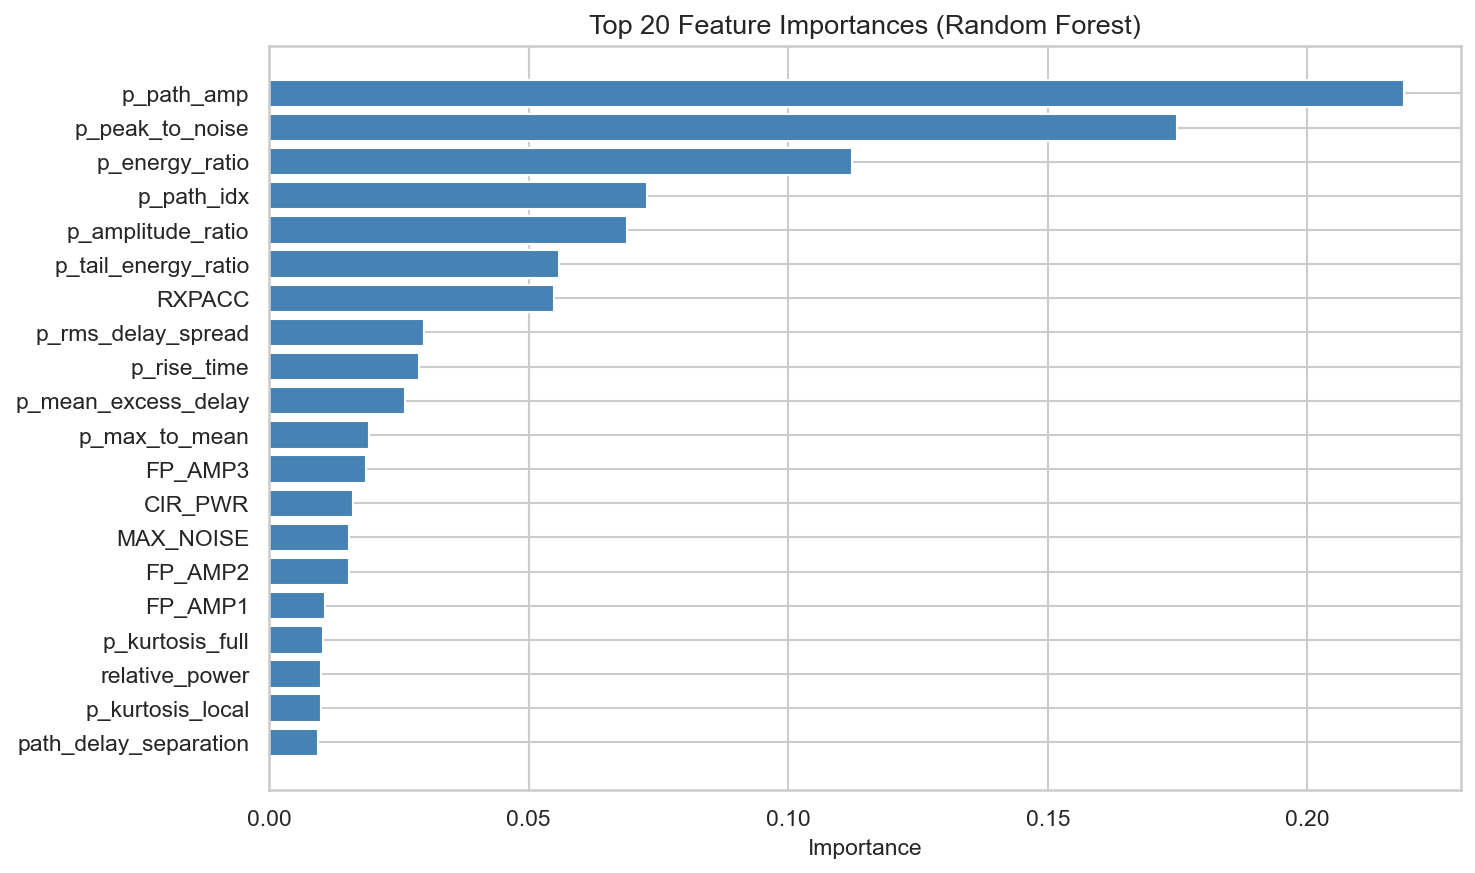
\includegraphics[width=\columnwidth]{06_feature_importance.png}
\caption{Top 15 features ranked by Random Forest Gini importance. Signal power and noise-related features dominate.}
\label{fig:importance}
\end{figure}

Classical ML baselines are trained on the engineered feature vectors: Logistic Regression (LR), SVM, Random Forest (RF), Gradient Boosted Trees (GBT), and XGBoost~\cite{b8}. We also evaluate simple probability averaging and stacked generalization on the strongest tree-based models.

\subsection{End-to-End Deep Learning Pipeline}

We propose a hybrid 1D-CNN + Transformer architecture that operates directly on the raw 1016-sample CIR waveform. Algorithm~\ref{alg:training} describes the training procedure.

\textbf{Architecture.} The model consists of three components:

\textit{1) Multi-scale CNN encoder:} Three convolutional blocks (Conv1D $\rightarrow$ BatchNorm $\rightarrow$ ReLU $\rightarrow$ MaxPool) progressively extract local patterns. The kernel sizes (7, 5, 3) are chosen to operate at multiple temporal scales: larger kernels capture broad multipath envelope patterns spanning several nanoseconds, while smaller kernels resolve fine-grained amplitude peaks characteristic of direct-path arrivals. The output is a sequence of 127 feature vectors of dimension 128.

\textit{2) Transformer encoder:} Two Transformer encoder layers with 4-head self-attention model global dependencies across the CNN-encoded sequence. Sinusoidal positional encoding preserves temporal ordering. The self-attention mechanism allows the model to relate distant CIR components, capturing multipath relationships that span the full waveform.

\textit{3) Classification head:} Global average pooling reduces the transformer output to a single 128-dimensional vector, which is concatenated with 11 scaled scalar features and passed through a two-layer MLP (hidden size 64) to produce a binary logit.

\begin{table}[t]
\caption{CNN-Transformer Hyperparameters}
\label{tab:hyperparams}
\centering
\begin{tabular}{@{}ll@{}}
\toprule
\textbf{Parameter} & \textbf{Value} \\
\midrule
CNN channels & 32 $\rightarrow$ 64 $\rightarrow$ 128 \\
CNN kernel sizes & 7, 5, 3 \\
Transformer layers & 2 \\
Attention heads & 4 \\
Feedforward dim & 256 \\
MLP hidden & 64 \\
Dropout & 0.1 \\
Optimizer & Adam (lr = $1 \times 10^{-3}$) \\
Loss & BCEWithLogitsLoss \\
Batch size & 256 \\
Early stopping & patience = 10 \\
Device & Apple MPS (GPU) \\
\bottomrule
\end{tabular}
\end{table}

\begin{algorithm}[t]
\caption{CNN-Transformer Training}
\label{alg:training}
\begin{algorithmic}[1]
\REQUIRE Training set $\{(\mathbf{c}_i, \mathbf{s}_i, y_i)\}_{i=1}^{N}$ (CIR, scalars, label)
\ENSURE Trained model $f_\theta$
\STATE Initialize $f_\theta$ with random weights
\STATE $\text{best\_loss} \leftarrow \infty$; $\text{patience\_count} \leftarrow 0$
\FOR{epoch = 1 to 100}
    \FOR{each mini-batch $B$}
        \STATE $\hat{y} \leftarrow f_\theta(\mathbf{c}_B, \mathbf{s}_B)$
        \STATE $\mathcal{L} \leftarrow \text{BCEWithLogits}(\hat{y}, y_B)$
        \STATE Update $\theta$ via Adam with $\nabla_\theta \mathcal{L}$
    \ENDFOR
    \STATE Compute validation loss $\mathcal{L}_\text{val}$
    \IF{$\mathcal{L}_\text{val} < \text{best\_loss}$}
        \STATE $\text{best\_loss} \leftarrow \mathcal{L}_\text{val}$; save $\theta$; reset patience
    \ELSE
        \STATE $\text{patience\_count} \leftarrow \text{patience\_count} + 1$
    \ENDIF
    \IF{$\text{patience\_count} \geq 10$}
        \STATE \textbf{break} (early stopping)
    \ENDIF
\ENDFOR
\RETURN $f_\theta$ with best validation weights
\end{algorithmic}
\end{algorithm}

The DL model is trained on the original balanced 42,000-sample dataset (not the two-path expanded set), using 80/20 stratified split. Training was performed on Apple MPS GPU acceleration and early-stopped at epoch 24.

%======================================================================
\section{Experimental Results}

\subsection{Classification Results}

Table~\ref{tab:cls_results} summarizes the classification results. The feature-engineered ML models are evaluated on the expanded two-path test set, whereas the CNN+Transformer results come from a separate raw-CIR pipeline evaluated on the original split. Therefore, the ML and DL rows are not a direct apples-to-apples comparison.

\begin{table}[t]
\caption{Classification Performance}
\label{tab:cls_results}
\centering
\begin{tabular}{@{}lccc@{}}
\toprule
\textbf{Model} & \textbf{Accuracy} & \textbf{AUC} & \textbf{Test Set} \\
\midrule
Logistic Regression & 0.9199 & 0.9694 & Expanded \\
SVM & 0.6523 & 0.8734 & Expanded \\
Random Forest & 0.9386 & 0.9815 & Expanded \\
Gradient Boosted Trees & 0.9311 & 0.9819 & Expanded \\
XGBoost & 0.9404 & 0.9834 & Expanded \\
Ensemble Avg & 0.9402 & 0.9831 & Expanded \\
Ensemble Stacked & 0.9415 & 0.9830 & Expanded \\
CNN+Transformer & 0.9360 & 0.9821 & Original split \\
CNN+Transformer + CIR Aug & 0.9421 & 0.9845 & Separate pipeline \\
\bottomrule
\end{tabular}
\end{table}

Among the directly comparable feature-engineered models, XGBoost gives the strongest single-model result (0.9404 accuracy, 0.9834 AUC), while stacked ensembling only slightly improves accuracy to 0.9415 without improving AUC. The SVM baseline is clearly weaker, indicating that the boundary is not well captured by that configuration. The raw-CIR CNN+Transformer is competitive in AUC, but because it is trained and evaluated in a separate pipeline on the original split, its numbers should be interpreted as complementary rather than strictly comparable to the engineered-feature ML results. Fig.~\ref{fig:roc} shows the ROC curves, and Fig.~\ref{fig:confusion} shows the confusion matrices.

\begin{figure}[t]
\centering
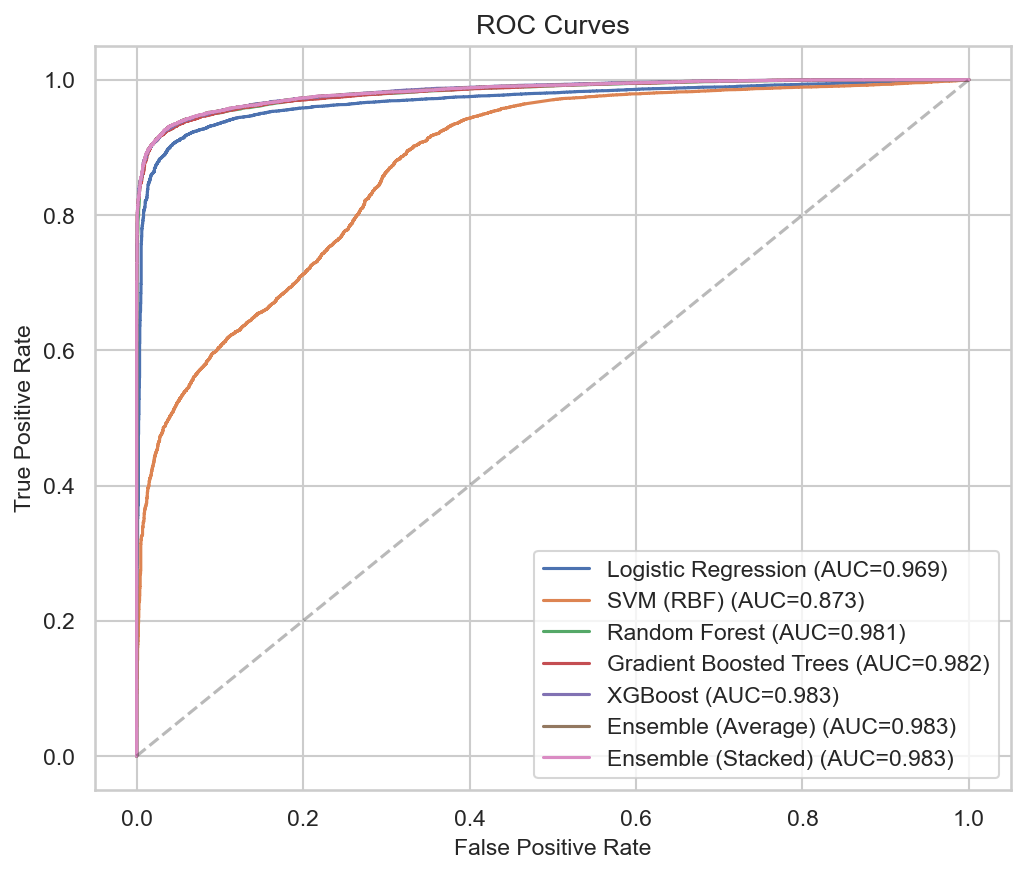
\includegraphics[width=\columnwidth]{08_roc_curves.png}
\caption{ROC curves for representative classification models. The strongest supervised models all achieve high AUC, but the DL rows come from a separate raw-CIR pipeline.}
\label{fig:roc}
\end{figure}

\begin{figure}[t]
\centering
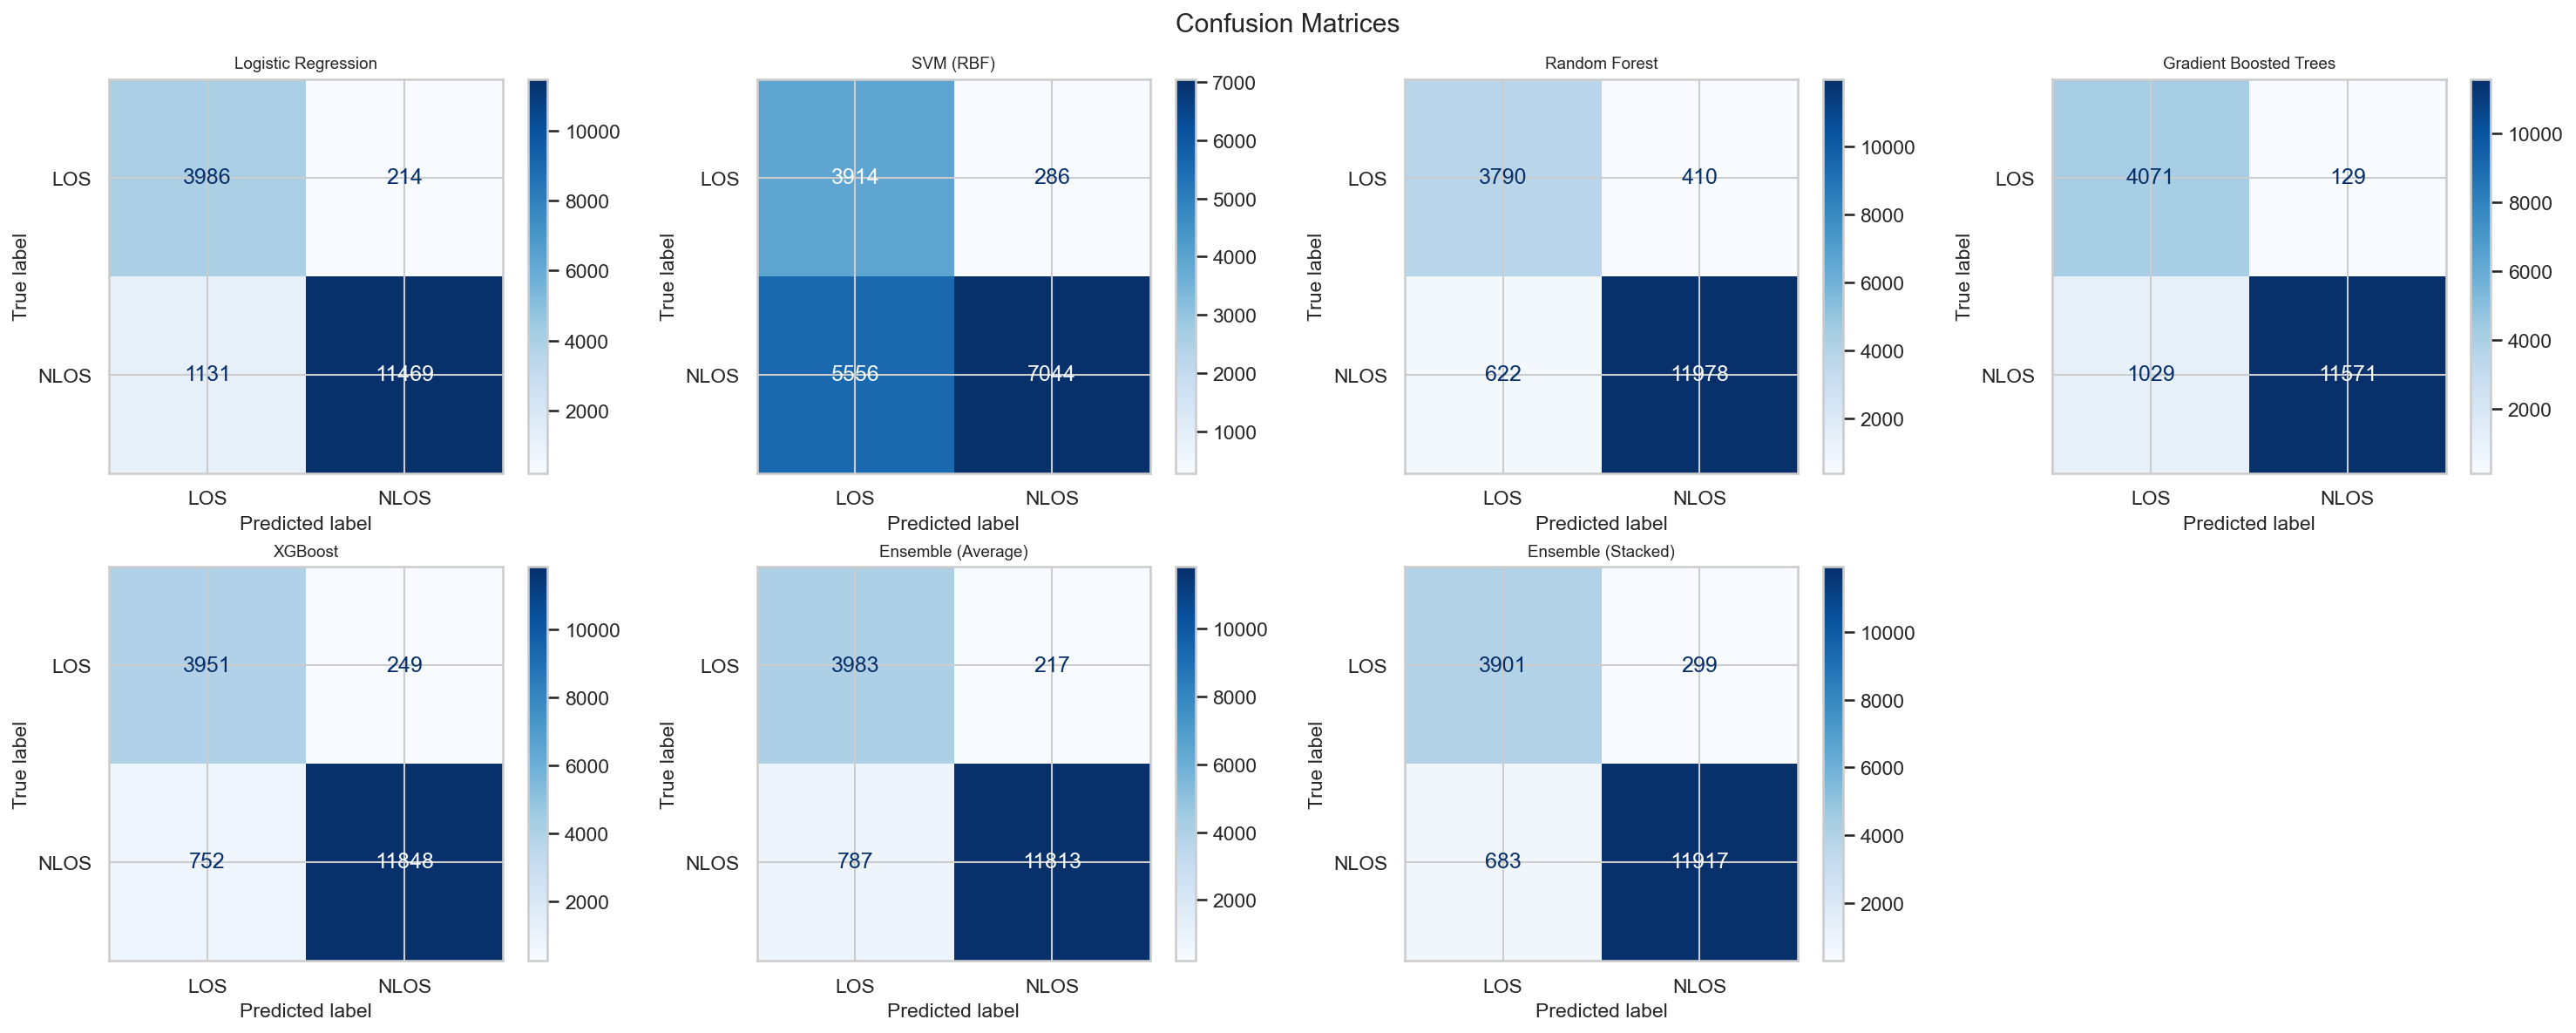
\includegraphics[width=\columnwidth]{07_confusion_matrices.png}
\caption{Confusion matrices for representative baseline classification models.}
\label{fig:confusion}
\end{figure}

\subsection{Distance Estimation Results}

Table~\ref{tab:reg_results} presents regression performance for both signal paths. Path~2 regression is reported on 8,193 valid test samples.

\begin{table}[t]
\caption{Distance Estimation Performance}
\label{tab:reg_results}
\centering
\begin{tabular}{@{}llcc@{}}
\toprule
\textbf{Path} & \textbf{Model} & \textbf{RMSE (m)} & \textbf{$R^2$} \\
\midrule
\multirow{4}{*}{Path 1} & Ridge & 1.6164 & 0.5407 \\
 & Random Forest & 1.3706 & 0.6698 \\
 & Gradient Boosted & 1.3872 & 0.6617 \\
 & XGBoost & 1.3726 & 0.6688 \\
\midrule
\multirow{4}{*}{Path 2} & Ridge & 0.0000 & 1.0000 \\
 & Random Forest & 0.4696 & 0.9997 \\
 & Gradient Boosted & 0.2889 & 0.9999 \\
 & XGBoost & 1.2176 & 0.9981 \\
\bottomrule
\end{tabular}
\end{table}

Path~1 regression is the more meaningful prediction task: the best models reach RMSE near 1.37\,m with $R^2\approx0.67$, indicating moderate but useful predictive value. By contrast, path~2 regression is analytically constrained because the target is defined from $\text{RANGE} + (\text{path2\_idx} - \text{FP\_IDX}) \cdot c$, and RANGE is also an input feature. The near-perfect path~2 scores therefore should not be interpreted as evidence of a genuinely difficult forecasting problem being solved. Fig.~\ref{fig:regression} shows predicted vs. actual distance scatter plots, and Fig.~\ref{fig:residuals} shows the residual distributions for both paths.

\begin{figure}[t]
\centering
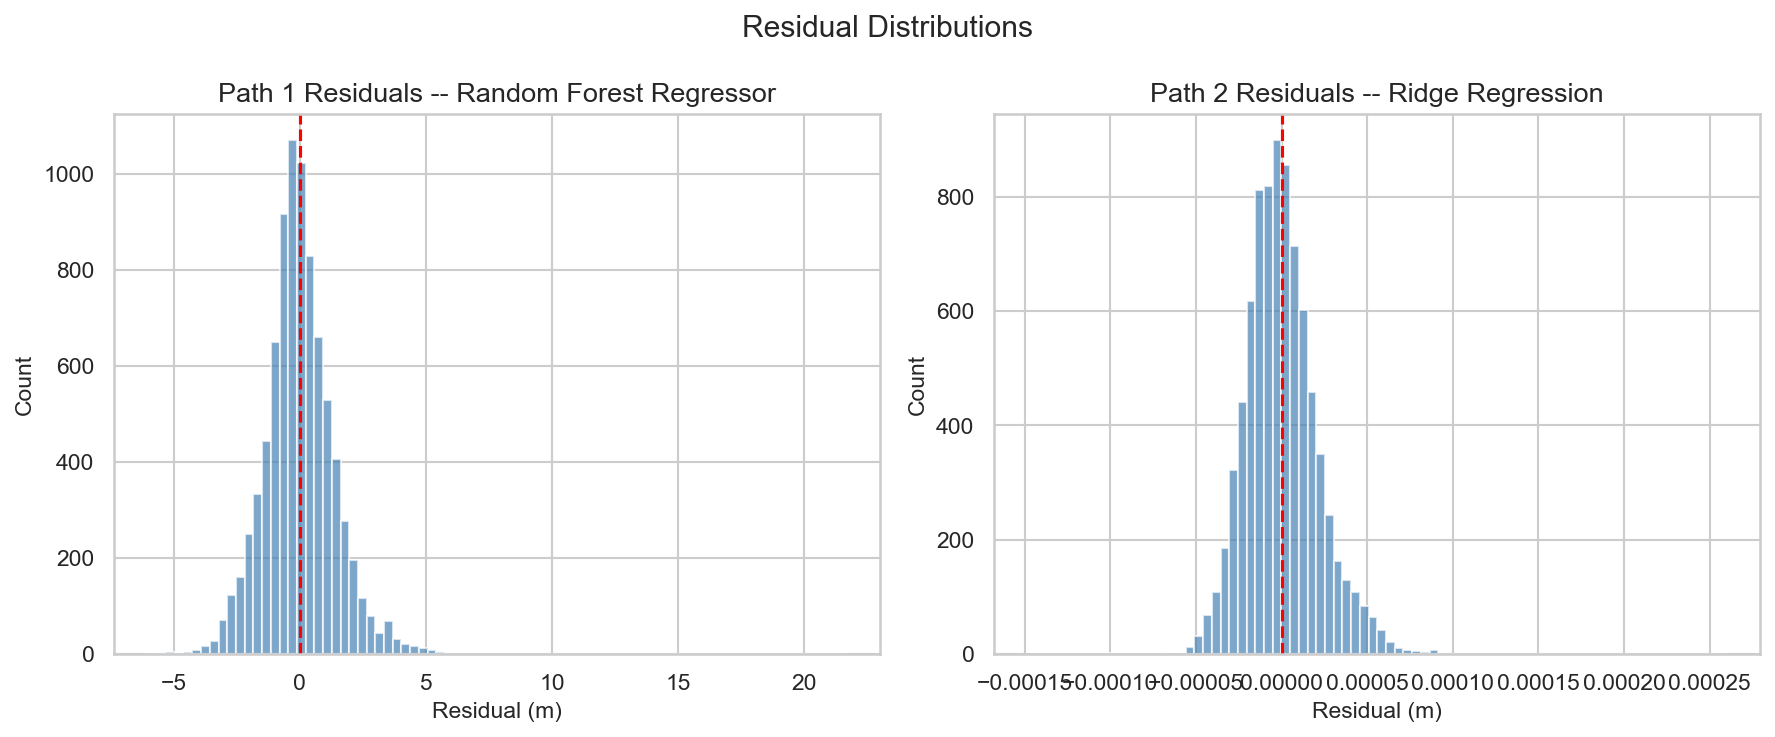
\includegraphics[width=\columnwidth]{11_residuals.png}
\caption{Residual distributions for distance estimation. Path~2 residuals are tightly concentrated around zero, consistent with its high $R^2$.}
\label{fig:residuals}
\end{figure}

\begin{figure}[t]
\centering
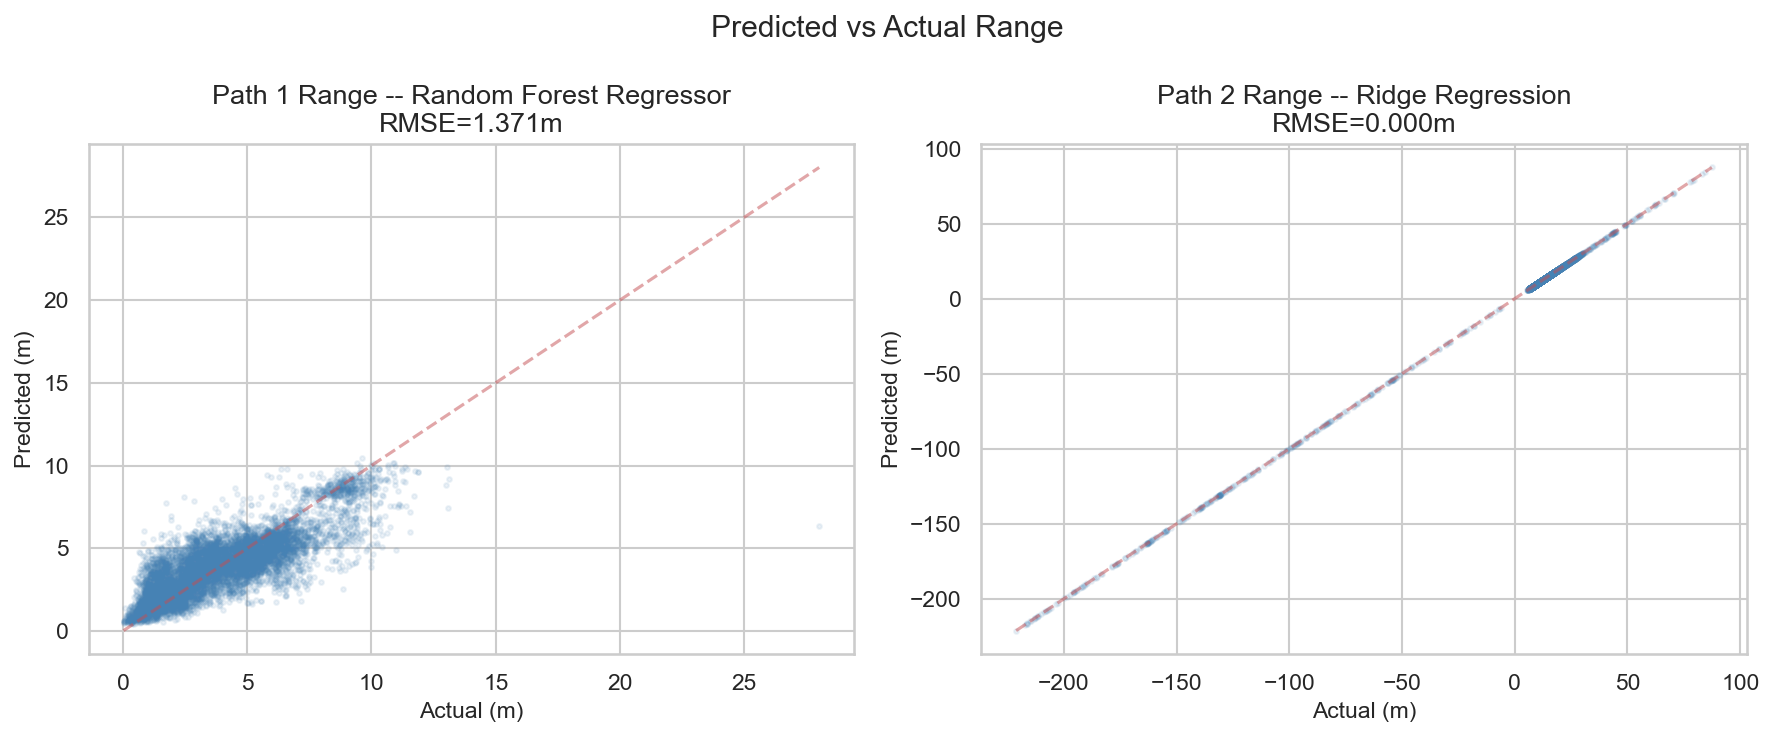
\includegraphics[width=\columnwidth]{10_predicted_vs_actual.png}
\caption{Predicted vs. actual distance for path 1 (left) and path 2 (right) regression models.}
\label{fig:regression}
\end{figure}

\subsection{Unsupervised Baseline}

As an unsupervised baseline, K-Means clustering ($k=2$) was applied to the Path~1-only feature set, not to the expanded two-path dataset. This correction is necessary because the expanded dataset is dominated by NLOS labels by construction. Before clustering, the engineered features were standardized with StandardScaler because both K-Means and PCA are distance-based and sensitive to feature scale. Even after optimal cluster-to-label mapping, K-Means is weak, achieving only 0.5906 test accuracy and ARI of 0.0269. DBSCAN performs worse still, producing 0 clusters and treating 100\% of test points as noise.

These results indicate that unsupervised separation of LOS and NLOS is weak in this feature space and should not be overstated. PCA can still be useful for visualization, but the clustering outcomes do not support strong claims about naturally separable structure.

\subsection{Ensemble Methods}

Two ensemble strategies combine the RF, GBT, and XGBoost classifiers. Simple probability averaging reaches 0.9402 accuracy and 0.9831 AUC, while stacked generalization reaches 0.9415 accuracy and 0.9830 AUC. The gain over the best single model is therefore marginal.

\subsection{Synthetic Data Augmentation}

We evaluate two augmentation strategies: SMOTE for the feature-engineered ML pipeline and CIR waveform augmentation (Gaussian noise injection, temporal jitter, amplitude scaling) for the CNN-Transformer. SMOTE generates synthetic minority-class samples in feature space, whereas CIR augmentation perturbs raw waveforms in the separate deep-learning pipeline.

CIR augmentation creates physically-motivated synthetic waveforms by perturbing real signals with additive noise ($\sigma = 0.08$), random temporal shifts ($\pm4$ samples), and amplitude scaling (0.80--1.20$\times$). These perturbations simulate receiver thermal noise, clock synchronisation imprecision, and path loss variation.

SMOTE has negligible effect on the classical ML results. The deep-learning augmentation is more noticeable, improving the separate CNN+Transformer pipeline from 0.9360/0.9821 to 0.9421/0.9845, but this remains a separate raw-CIR pipeline and should not be read as a direct augmentation comparison against the feature-engineered ML models.

%======================================================================
\section{Discussion}

\subsection{ML vs. Deep Learning Comparison}

The most notable finding is the close AUC range across the strongest supervised models: XGBoost reaches 0.9834 on the expanded two-path task, while the raw-CIR CNN+Transformer reaches 0.9821 and 0.9845 with augmentation in its separate pipeline. This suggests that both engineered features and end-to-end raw-CIR learning capture substantial LOS/NLOS signal structure. Fig.~\ref{fig:comparison} summarizes the model comparison.

The accuracy difference should be interpreted with caution because the ML and DL pipelines are not evaluated on the same task formulation or split: the ML results come from the expanded two-path dataset, while the DL results come from a separate raw-CIR pipeline on the original split. Accordingly, the ML-vs-DL comparison is informative at a high level but not a strict apples-to-apples benchmark.

The ensemble gains are also small, suggesting that most of the recoverable supervised signal is already captured by the best tree-based learner. A stricter ML-vs-DL comparison would require retraining both pipelines on the same split and label construction.

\begin{figure}[t]
\centering
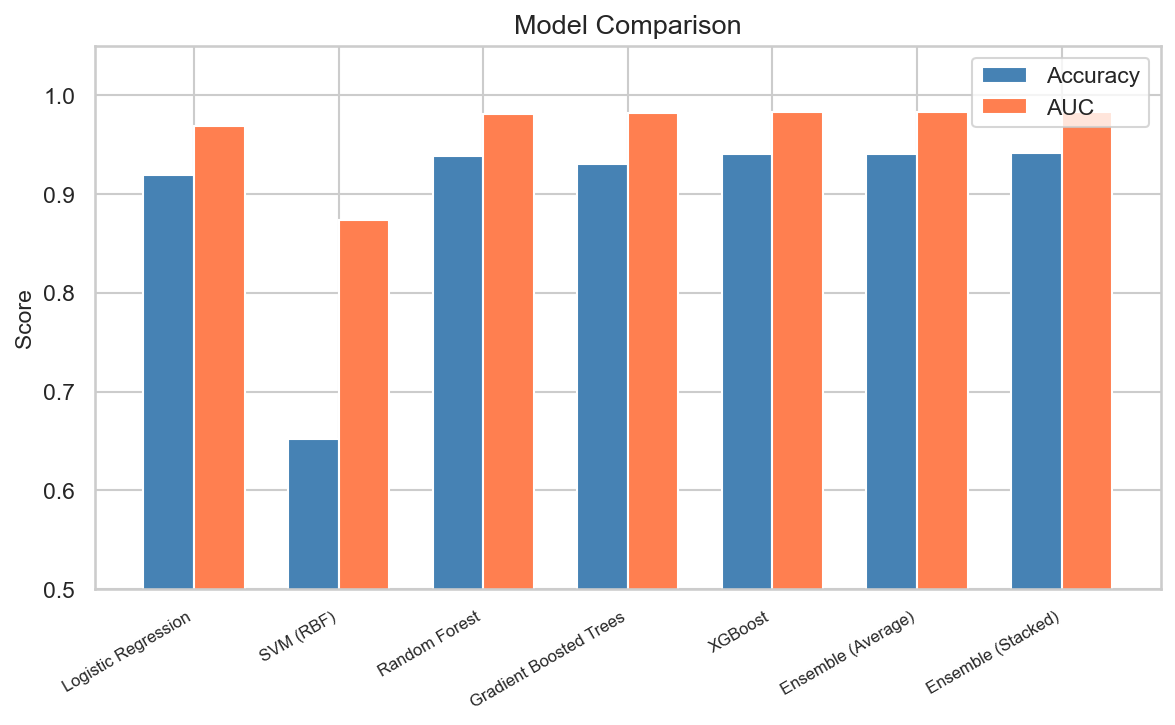
\includegraphics[width=\columnwidth]{09_model_comparison.png}
\caption{Comparison of classification metrics across all models.}
\label{fig:comparison}
\end{figure}

\subsection{Interpretability via Attention}

A key advantage of the CNN-Transformer is interpretability through attention weight visualization. Fig.~\ref{fig:annotated_cir} shows an annotated CIR waveform with the physical regions of interest, while Fig.~\ref{fig:attention} shows the attention pattern learned by the model. The Transformer's self-attention heads focus on regions near the first path arrival and secondary reflections, aligning with the physical interpretation of multipath propagation. This provides insight into which CIR regions drive the model's decisions, complementing the feature importance analysis of classical models.

\begin{figure}[t]
\centering
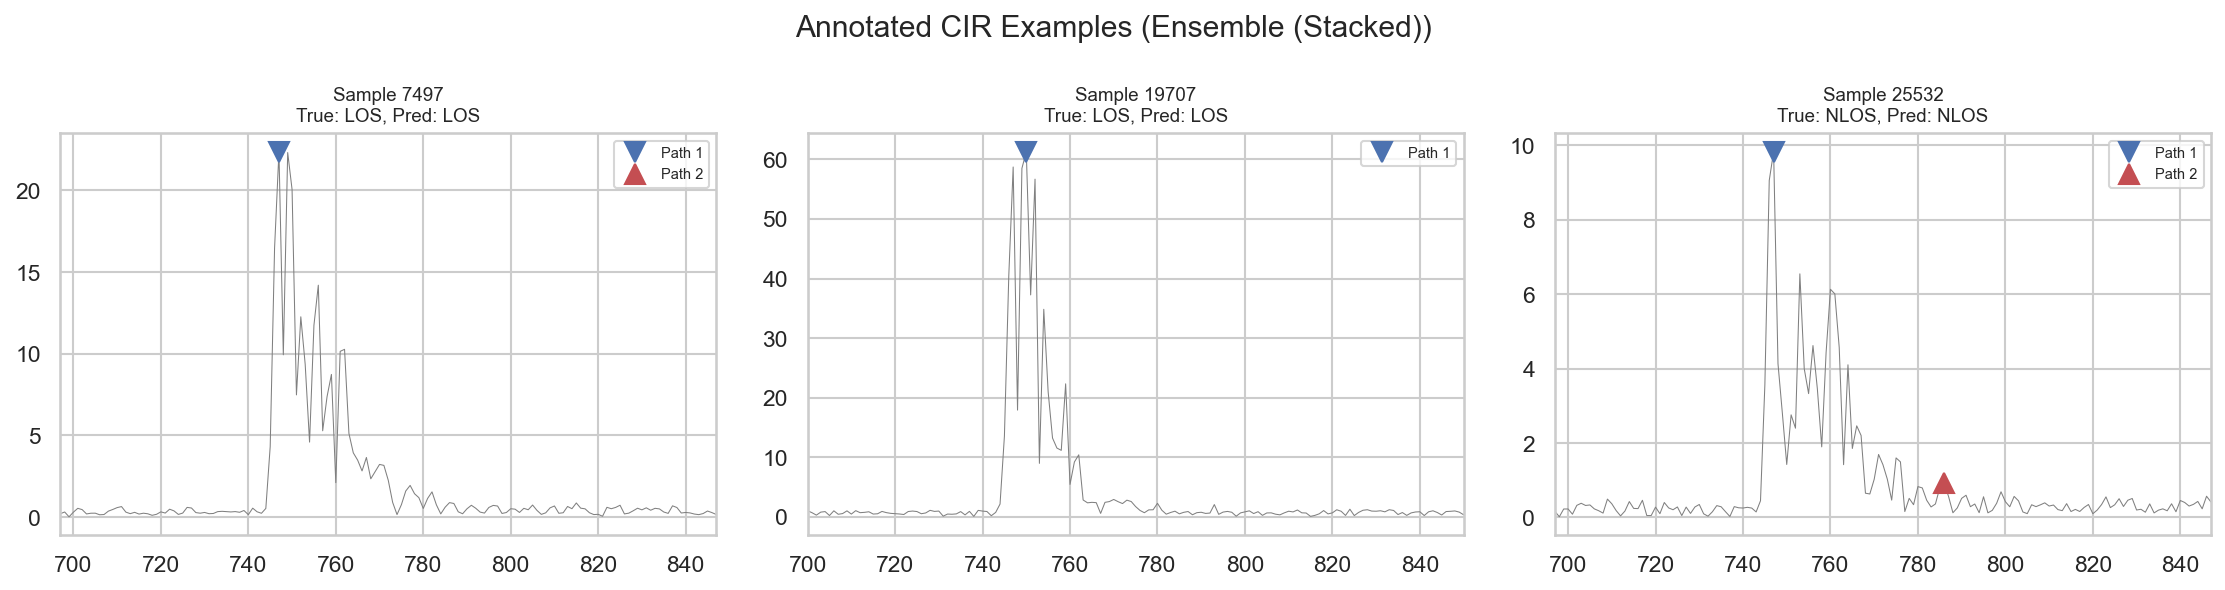
\includegraphics[width=\columnwidth]{12_annotated_cir.png}
\caption{Annotated CIR waveform highlighting the first path, second path, and noise floor regions used for feature extraction.}
\label{fig:annotated_cir}
\end{figure}

\begin{figure}[t]
\centering
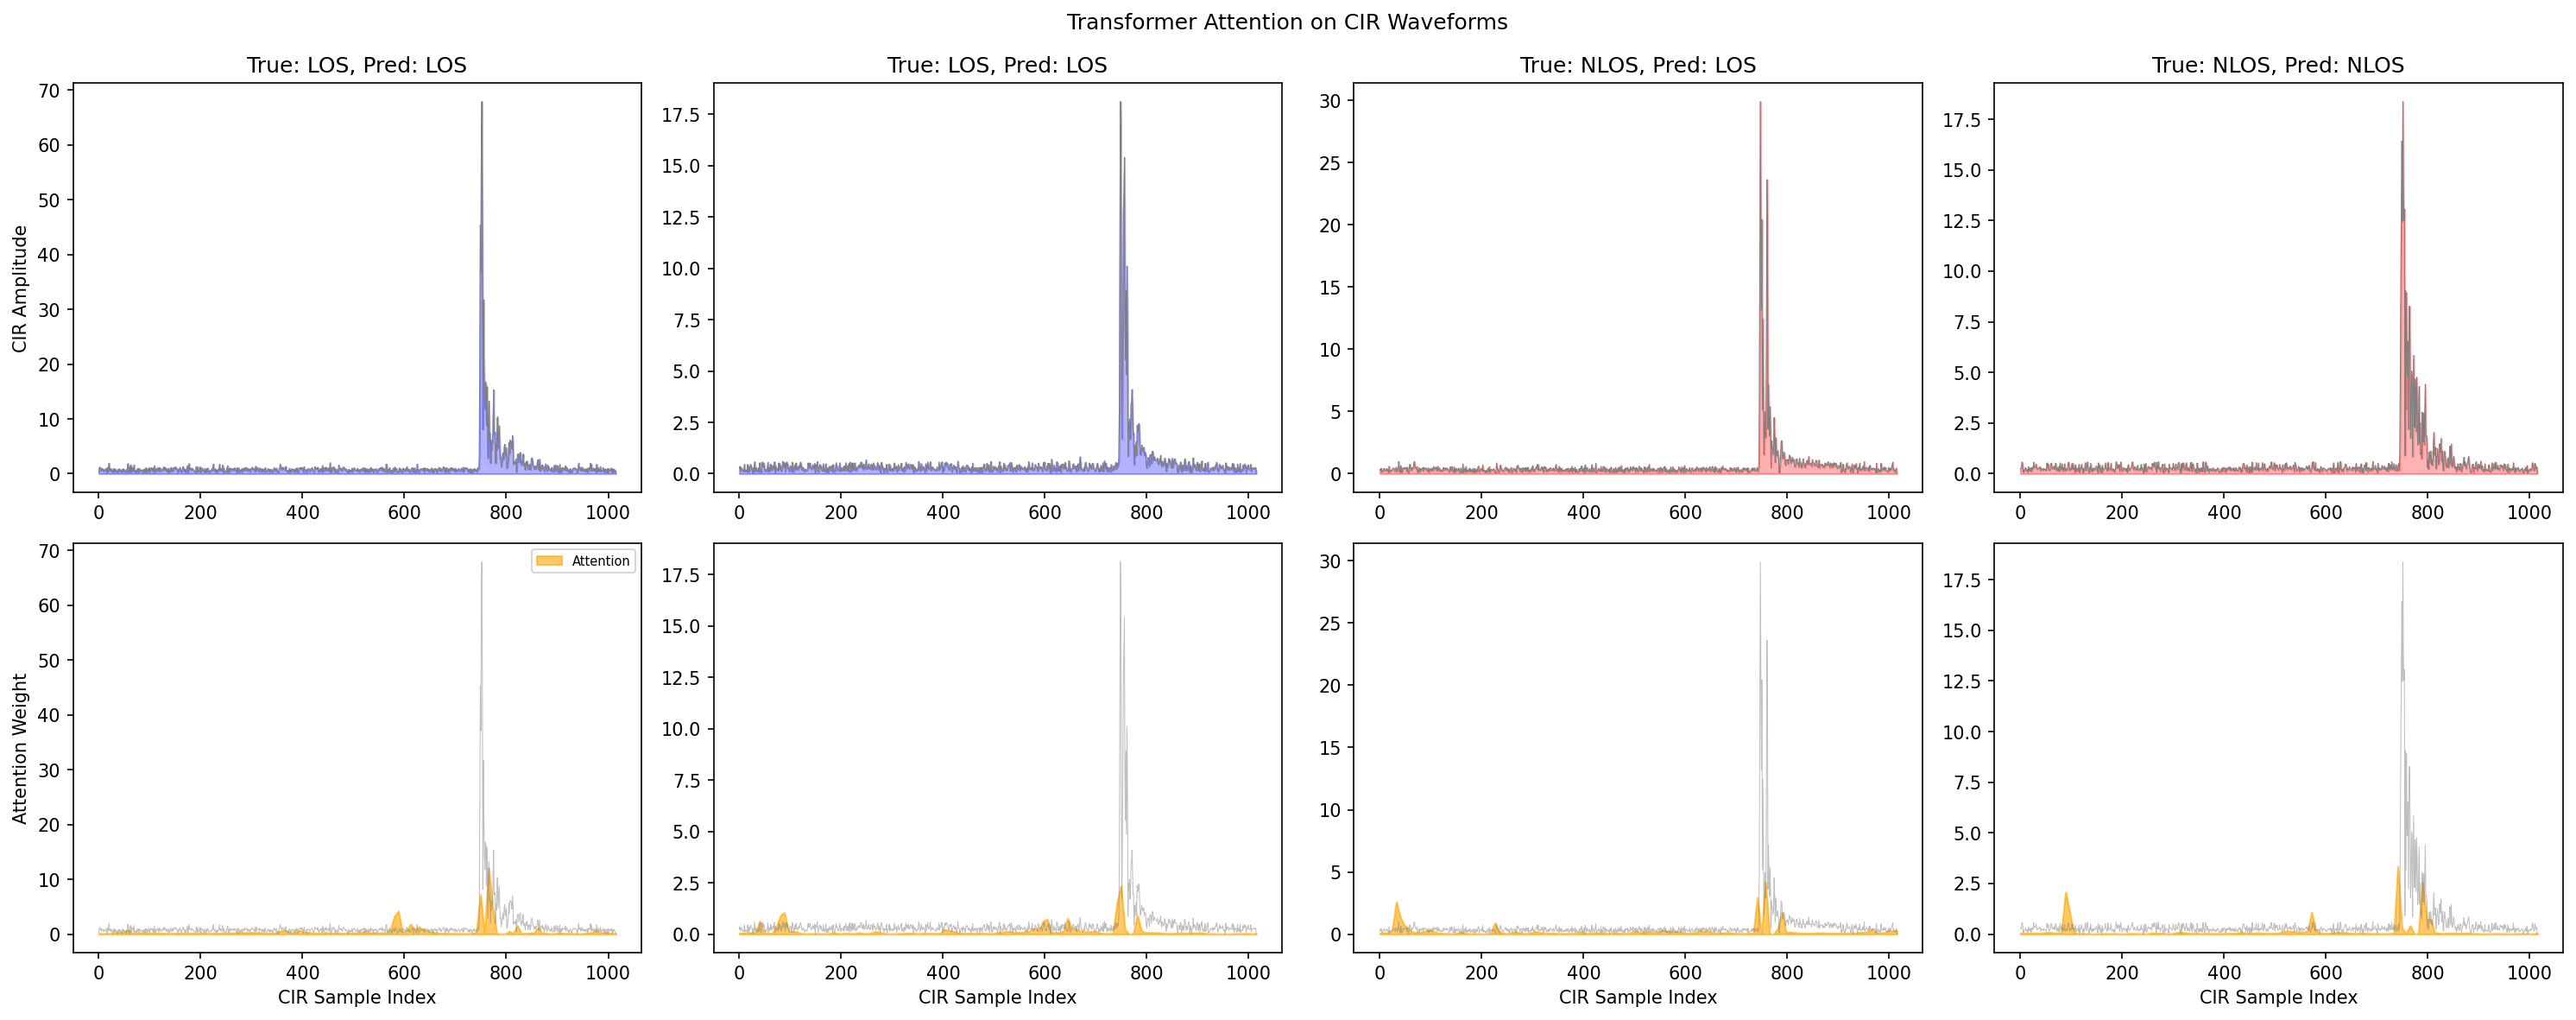
\includegraphics[width=\columnwidth]{13_attention_map.png}
\caption{Transformer attention weights overlaid on a CIR waveform. High attention concentrates near the first path and multipath components.}
\label{fig:attention}
\end{figure}

\subsection{Error Analysis}

Classification errors primarily occur in ambiguous cases where NLOS signals have strong direct-path-like characteristics or where LOS signals experience significant multipath interference. The weaker LR and SVM baselines (AUC 0.9694 and 0.8734) indicate that the LOS/NLOS boundary is not well captured by simpler decision surfaces.

For distance estimation, path~1 regression is more challenging because the measured range includes environment-dependent NLOS bias that is not fully determined by the engineered predictors. Path~2 regression, in contrast, is partly tautological because the target is constructed from timing information and RANGE that are already present in the inputs.

\subsection{Model Complexity}

Table~\ref{tab:complexity} compares model complexity. The CNN-Transformer has substantially more parameters but offers the advantage of requiring no manual feature engineering.

\begin{table}[t]
\caption{Model Complexity Comparison}
\label{tab:complexity}
\centering
\begin{tabular}{@{}lcc@{}}
\toprule
\textbf{Model} & \textbf{Input Dim} & \textbf{Feature Eng.} \\
\midrule
Logistic Regression & 25 & Yes (manual) \\
Random Forest & 25 & Yes (manual) \\
Gradient Boosted Trees & 25 & Yes (manual) \\
XGBoost & 25 & Yes (manual) \\
CNN-Transformer & 1016 + 11 & No (end-to-end) \\
\bottomrule
\end{tabular}
\end{table}

%======================================================================
\section{Conclusion}

We presented a concise framework for UWB LOS/NLOS classification and distance estimation using a feature-engineered ML pipeline and a separate raw-CIR CNN+Transformer pipeline. After preprocessing, two-path extraction recovered a second path in 97.3\% of valid samples and expanded the supervised feature-engineered dataset to 83,992 rows.

Key findings include: (1) XGBoost is the strongest directly comparable ML classifier at 0.9404 accuracy and 0.9834 AUC, with only marginal additional benefit from ensembling; (2) the CNN+Transformer is competitive, but its results come from a separate raw-CIR pipeline on the original split, so ML-vs-DL claims should remain cautious; (3) path~1 regression is moderately effective, whereas path~2 regression is heavily constrained by how the target is defined and should not be over-interpreted; and (4) unsupervised clustering is weak, so the main evidence in this study comes from supervised learning rather than natural class separation.

\subsection{Future Work}

Several directions merit further investigation: (1) Ensemble methods combining ML and DL predictions, potentially using the CNN-Transformer as an additional base learner alongside tree-based models; (2) Cross-environment generalization studies using leave-one-environment-out validation to assess domain shift; (3) Model compression and quantization for real-time deployment on embedded UWB receivers; (4) Extension to multi-class scenarios distinguishing between different NLOS propagation mechanisms (diffraction, reflection, scattering); (5) Cross-domain transfer learning, where models pre-trained on one indoor environment are fine-tuned on a new environment with limited labeled data, reducing the data collection burden for practical deployments.

\section*{Acknowledgment}

The authors thank the contributors of the UWB-LOS-NLOS-Data-Set for making the dataset publicly available.

\begin{thebibliography}{00}
\bibitem{b1} Z. Sahinoglu, S. Gezici, and I. Guvenc, ``Ultra-wideband positioning systems: theoretical limits, ranging algorithms, and protocols,'' Cambridge University Press, 2008.
\bibitem{b2} H. Wymeersch, J. Lien, and M. Z. Win, ``Cooperative localization in wireless networks,'' \textit{Proc. IEEE}, vol. 97, no. 2, pp. 427--450, Feb. 2009.
\bibitem{b3} J. Khodjaev, Y. Park, and A. S. Malik, ``Survey of NLOS identification and error mitigation problems in UWB-based positioning algorithms for dense environments,'' \textit{Ann. Telecommun.}, vol. 65, pp. 301--311, 2010.
\bibitem{b4} S. Marano, W. M. Gifford, H. Wymeersch, and M. Z. Win, ``NLOS identification and mitigation for localization based on UWB experimental data,'' \textit{IEEE J. Sel. Areas Commun.}, vol. 28, no. 7, pp. 1026--1035, Sep. 2010.
\bibitem{b5} A. Niitsoo, T. Edelhausser, E. Eberlein, N. Hadaschik, and C. Mutschler, ``A deep learning approach to position estimation from channel impulse responses,'' \textit{Sensors}, vol. 19, no. 5, p. 1064, 2019.
\bibitem{b6} A. Vaswani, N. Shazeer, N. Parmar, J. Uszkoreit, L. Jones, A. N. Gomez, L. Kaiser, and I. Polosukhin, ``Attention is all you need,'' in \textit{Proc. NeurIPS}, 2017, pp. 5998--6008.
\bibitem{b7} K. Bregar and M. Mohorcic, ``Improving indoor localization using convolutional neural networks on computationally restricted devices,'' \textit{IEEE Access}, vol. 6, pp. 17429--17441, 2018.
\bibitem{b8} T. Chen and C. Guestrin, ``XGBoost: a scalable tree boosting system,'' in \textit{Proc. ACM SIGKDD}, 2016, pp. 785--794.
\bibitem{b9} L. Breiman, ``Random forests,'' \textit{Machine Learning}, vol. 45, no. 1, pp. 5--32, 2001.
\bibitem{b10} J. Devlin, M.-W. Chang, K. Lee, and K. Toutanova, ``BERT: pre-training of deep bidirectional transformers for language understanding,'' in \textit{Proc. NAACL-HLT}, 2019, pp. 4171--4186.
\bibitem{b11} S. Tomović, K. Bregar, T. Javornik, and M. Mohorčič, ``Transformer-based NLoS detection in UWB localization systems,'' in \textit{Proc. 30th Telecommun. Forum (TELFOR)}, 2022.
\bibitem{b12} H. J. Hwang, S. G. Jeong, and W. J. Hwang, ``Ultrawideband non-line-of-sight classification using transformer-convolutional neural networks,'' \textit{IEEE Access}, 2025.
\end{thebibliography}

\end{document}
